\section{Introducción}
Escribe aquí la introducción de tu documento. Este documento sigue un estilo parecido a la serie Lecture Notes in Computer Science (LNCS).

\section{Trabajo Relacionado}
Describe aquí el trabajo relacionado con el tema de tu documento. Puedes citar trabajos previos usando comandos como \cite{lamport1994latex}.

\section{Metodología}
Detalla la metodología que has seguido para llevar a cabo tu investigación o estudio.

\section{Resultados}
Presenta aquí los resultados obtenidos. Puedes incluir figuras, tablas y ecuaciones.

\subsection{Tabla}
Y aquí incluimos una tabla como ejemplo:

\begin{table}[htbp]
  \centering
  \caption{Ejemplo de tabla}
  \label{tab:ejemplo}
  \begin{tabular}{|c|c|}
    \hline
    \textbf{Columna 1} & \textbf{Columna 2} \\
    \hline
    Valor 1 & Valor A \\
    Valor 2 & Valor B \\
    \hline
  \end{tabular}
\end{table}

\subsection{Figura}
Aquí incluimos una figura como ejemplo:

\begin{figure}[htbp]
  \centering
  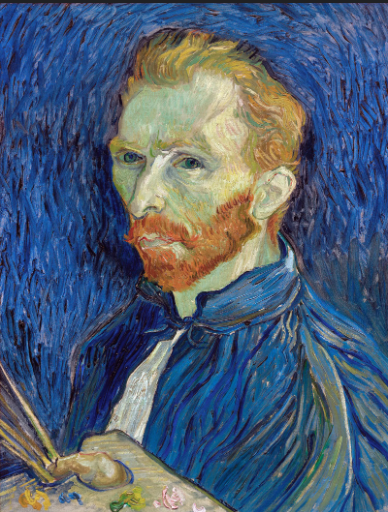
\includegraphics[width=5cm]{./assets/images/ejemplo.png} % Cambia 'ejemplo_figura.png' por el nombre de tu archivo de imagen
  \caption{Descripción de la figura.}
  \label{fig:ejemplo}
\end{figure}

\section{Conclusiones}
Escribe las conclusiones a las que has llegado con tu estudio o investigación. También puedes discutir posibles trabajos futuros~\cite{knuth1997art}.

\section*{Agradecimientos}
Incluye los agradecimientos, si es necesario.
\bibliographystyle{splncs04}
